% Options for packages loaded elsewhere
\PassOptionsToPackage{unicode}{hyperref}
\PassOptionsToPackage{hyphens}{url}
\PassOptionsToPackage{dvipsnames,svgnames,x11names}{xcolor}
%
\documentclass[
  letterpaper,
  DIV=11,
  numbers=noendperiod]{scrreprt}

\usepackage{amsmath,amssymb}
\usepackage{iftex}
\ifPDFTeX
  \usepackage[T1]{fontenc}
  \usepackage[utf8]{inputenc}
  \usepackage{textcomp} % provide euro and other symbols
\else % if luatex or xetex
  \usepackage{unicode-math}
  \defaultfontfeatures{Scale=MatchLowercase}
  \defaultfontfeatures[\rmfamily]{Ligatures=TeX,Scale=1}
\fi
\usepackage{lmodern}
\ifPDFTeX\else  
    % xetex/luatex font selection
\fi
% Use upquote if available, for straight quotes in verbatim environments
\IfFileExists{upquote.sty}{\usepackage{upquote}}{}
\IfFileExists{microtype.sty}{% use microtype if available
  \usepackage[]{microtype}
  \UseMicrotypeSet[protrusion]{basicmath} % disable protrusion for tt fonts
}{}
\makeatletter
\@ifundefined{KOMAClassName}{% if non-KOMA class
  \IfFileExists{parskip.sty}{%
    \usepackage{parskip}
  }{% else
    \setlength{\parindent}{0pt}
    \setlength{\parskip}{6pt plus 2pt minus 1pt}}
}{% if KOMA class
  \KOMAoptions{parskip=half}}
\makeatother
\usepackage{xcolor}
\setlength{\emergencystretch}{3em} % prevent overfull lines
\setcounter{secnumdepth}{5}
% Make \paragraph and \subparagraph free-standing
\ifx\paragraph\undefined\else
  \let\oldparagraph\paragraph
  \renewcommand{\paragraph}[1]{\oldparagraph{#1}\mbox{}}
\fi
\ifx\subparagraph\undefined\else
  \let\oldsubparagraph\subparagraph
  \renewcommand{\subparagraph}[1]{\oldsubparagraph{#1}\mbox{}}
\fi


\providecommand{\tightlist}{%
  \setlength{\itemsep}{0pt}\setlength{\parskip}{0pt}}\usepackage{longtable,booktabs,array}
\usepackage{calc} % for calculating minipage widths
% Correct order of tables after \paragraph or \subparagraph
\usepackage{etoolbox}
\makeatletter
\patchcmd\longtable{\par}{\if@noskipsec\mbox{}\fi\par}{}{}
\makeatother
% Allow footnotes in longtable head/foot
\IfFileExists{footnotehyper.sty}{\usepackage{footnotehyper}}{\usepackage{footnote}}
\makesavenoteenv{longtable}
\usepackage{graphicx}
\makeatletter
\def\maxwidth{\ifdim\Gin@nat@width>\linewidth\linewidth\else\Gin@nat@width\fi}
\def\maxheight{\ifdim\Gin@nat@height>\textheight\textheight\else\Gin@nat@height\fi}
\makeatother
% Scale images if necessary, so that they will not overflow the page
% margins by default, and it is still possible to overwrite the defaults
% using explicit options in \includegraphics[width, height, ...]{}
\setkeys{Gin}{width=\maxwidth,height=\maxheight,keepaspectratio}
% Set default figure placement to htbp
\makeatletter
\def\fps@figure{htbp}
\makeatother
% definitions for citeproc citations
\NewDocumentCommand\citeproctext{}{}
\NewDocumentCommand\citeproc{mm}{%
  \begingroup\def\citeproctext{#2}\cite{#1}\endgroup}
\makeatletter
 % allow citations to break across lines
 \let\@cite@ofmt\@firstofone
 % avoid brackets around text for \cite:
 \def\@biblabel#1{}
 \def\@cite#1#2{{#1\if@tempswa , #2\fi}}
\makeatother
\newlength{\cslhangindent}
\setlength{\cslhangindent}{1.5em}
\newlength{\csllabelwidth}
\setlength{\csllabelwidth}{3em}
\newenvironment{CSLReferences}[2] % #1 hanging-indent, #2 entry-spacing
 {\begin{list}{}{%
  \setlength{\itemindent}{0pt}
  \setlength{\leftmargin}{0pt}
  \setlength{\parsep}{0pt}
  % turn on hanging indent if param 1 is 1
  \ifodd #1
   \setlength{\leftmargin}{\cslhangindent}
   \setlength{\itemindent}{-1\cslhangindent}
  \fi
  % set entry spacing
  \setlength{\itemsep}{#2\baselineskip}}}
 {\end{list}}
\usepackage{calc}
\newcommand{\CSLBlock}[1]{\hfill\break\parbox[t]{\linewidth}{\strut\ignorespaces#1\strut}}
\newcommand{\CSLLeftMargin}[1]{\parbox[t]{\csllabelwidth}{\strut#1\strut}}
\newcommand{\CSLRightInline}[1]{\parbox[t]{\linewidth - \csllabelwidth}{\strut#1\strut}}
\newcommand{\CSLIndent}[1]{\hspace{\cslhangindent}#1}

\KOMAoption{captions}{tableheading}
\makeatletter
\@ifpackageloaded{bookmark}{}{\usepackage{bookmark}}
\makeatother
\makeatletter
\@ifpackageloaded{caption}{}{\usepackage{caption}}
\AtBeginDocument{%
\ifdefined\contentsname
  \renewcommand*\contentsname{Table of contents}
\else
  \newcommand\contentsname{Table of contents}
\fi
\ifdefined\listfigurename
  \renewcommand*\listfigurename{List of Figures}
\else
  \newcommand\listfigurename{List of Figures}
\fi
\ifdefined\listtablename
  \renewcommand*\listtablename{List of Tables}
\else
  \newcommand\listtablename{List of Tables}
\fi
\ifdefined\figurename
  \renewcommand*\figurename{Figure}
\else
  \newcommand\figurename{Figure}
\fi
\ifdefined\tablename
  \renewcommand*\tablename{Table}
\else
  \newcommand\tablename{Table}
\fi
}
\@ifpackageloaded{float}{}{\usepackage{float}}
\floatstyle{ruled}
\@ifundefined{c@chapter}{\newfloat{codelisting}{h}{lop}}{\newfloat{codelisting}{h}{lop}[chapter]}
\floatname{codelisting}{Listing}
\newcommand*\listoflistings{\listof{codelisting}{List of Listings}}
\makeatother
\makeatletter
\makeatother
\makeatletter
\@ifpackageloaded{caption}{}{\usepackage{caption}}
\@ifpackageloaded{subcaption}{}{\usepackage{subcaption}}
\makeatother
\ifLuaTeX
  \usepackage{selnolig}  % disable illegal ligatures
\fi
\usepackage{bookmark}

\IfFileExists{xurl.sty}{\usepackage{xurl}}{} % add URL line breaks if available
\urlstyle{same} % disable monospaced font for URLs
\hypersetup{
  pdftitle={Medical Device Systems Engineering Knowledge Repository Report},
  pdfauthor={Esteban Solorzano},
  colorlinks=true,
  linkcolor={blue},
  filecolor={Maroon},
  citecolor={Blue},
  urlcolor={Blue},
  pdfcreator={LaTeX via pandoc}}

\title{Medical Device Systems Engineering Knowledge Repository Report}
\author{Esteban Solorzano}
\date{2024-04-02}

\begin{document}
\maketitle

\renewcommand*\contentsname{Table of contents}
{
\hypersetup{linkcolor=}
\setcounter{tocdepth}{2}
\tableofcontents
}
\bookmarksetup{startatroot}

\chapter*{Preface}\label{preface}
\addcontentsline{toc}{chapter}{Preface}

\markboth{Preface}{Preface}

This is a Quarto book.

To learn more about Quarto books visit
\url{https://quarto.org/docs/books}.

\bookmarksetup{startatroot}

\chapter{Introduction}\label{introduction}

This is a book created from markdown and executable code.

See Knuth (1984) for additional discussion of literate programming.

\bookmarksetup{startatroot}

\chapter{Summary}\label{summary}

This project delves into the intricacies of defining and managing
content in online reference books, particularly focusing on the domain
of medical device systems engineering. The study employs Systems
Engineering principles to analyze and propose a methodology for
efficiently defining content and a system for managing it.

\bookmarksetup{startatroot}

\chapter{Methodology}\label{methodology}

The study adopts a Systems Engineering approach, which involves
analyzing the entire content management process as a system with
interconnected components. This methodology allows for a holistic
understanding of the system's requirements, interactions, and potential
improvements. The research methodology encompasses:

\begin{enumerate}
\def\labelenumi{\arabic{enumi}.}
\tightlist
\item
  \textbf{Requirement Analysis:} Identifying the key requirements for
  efficient content management, including version control, compatibility
  with various file formats, and ease of collaboration.
\item
  \textbf{System Modeling:} Utilizing SysML (Systems Modeling Language)
  to create diagrams such as sequence diagrams, activity diagrams, and
  state machine diagrams to visualize the content management process and
  its interactions.
\item
  \textbf{Evaluation:} Assessing existing tools and technologies for
  content management, including Quatro and its capabilities in rendering
  content into different formats like HTML and PDF.
\item
  \textbf{Proposal:} Proposing a refined content management methodology
  tailored to the specific needs of online reference books in medical
  device systems engineering.
\end{enumerate}

\section{General methods}\label{general-methods}

The following methodology was used for the Masters Project in Systems
Engineering.

\begin{itemize}
\item
  Use Stevens Institute of Technology guidelines and templates for
  masters project.
\item
  Develop the ``knowledge repository'' as a system: stakeholder needs,
  concept, architecture, models, requirements, verification/validation.
\item
  Select and utilize systems engineering methods and tools from courses
  of Stevens School of Systems and Enterprises.
\item
  Select and utilize industry standards such as IEC 15288 and the INCOSE
  (International Council on Systems Engineering) Systems Engineering
  Handbook INCOSE (2023).
\item
  Literature Review: Conduct an extensive review of existing literature,
  research papers, and relevant resources in the field of systems
  engineering and medical devices.
\item
  Interviews and Surveys: Collect insights and best practices from
  industry experts, professionals, and academics in both systems
  engineering and medical device development.
\item
  Content Development: Create well-structured chapters and sections
  based on the outlined scope, ensuring clarity and coherence throughout
  the book.
\item
  Graphics and Illustrations: Include diagrams, flowcharts, and
  illustrations to enhance understanding and provide practical examples.
\item
  Peer Review: Seek input and feedback from experts in the field to
  validate the content's accuracy and relevance.
\item
  Use Git and/or GitHub as repository for the master's project
  artifacts.
\end{itemize}

\section{Systems Engineering Methods}\label{systems-engineering-methods}

\subsection{Systems Engineering Model}\label{systems-engineering-model}

\includegraphics[width=4.49in,height=6.65in]{methodology_files/figure-latex/mermaid-figure-1.png}

\bookmarksetup{startatroot}

\chapter{Operational Analysis}\label{operational-analysis}

\section{System Context}\label{system-context}

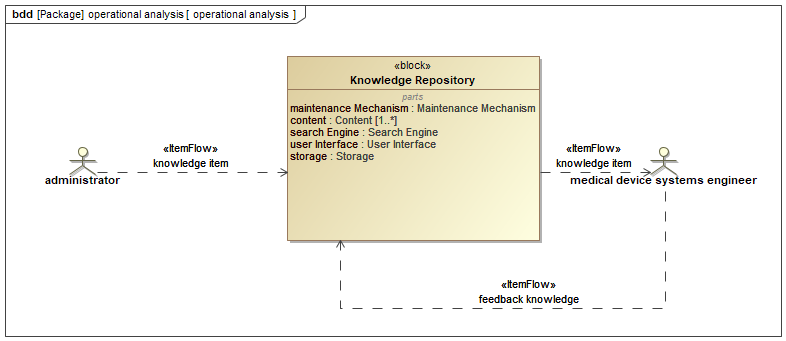
\includegraphics{images/paste-3.png}

This section defines the system context for the knowledge repository.
The analysis employs a SysML block definition diagram. The diagram
depicts a system centered around a knowledge repository containing
information relevant to medical services.

\subsection{Central Block: Knowledge
Repository}\label{central-block-knowledge-repository}

The core element of the system is the \textbf{Knowledge Repository}
block. This block represents a database or information storage system
that houses the medical device systems engineering knowledge base. The
knowledge base is comprised of multiple \textbf{Content} elements,
indicated by the notation ``{[}1..*{]}''. This multiplicity signifies
that the repository must contain at least one content element, and the
number of content elements can be limitless. The content would likely
encompasses details about regulatory, risk management, requirements
management, and other relevant medical device systems engineering
information.

The knowledge repository also includes a \textbf{Search Engine}
component. This component plays a critical role in facilitating
efficient retrieval of information from the content base. Users can
leverage the search engine to locate specific knowledge items based on
their needs.

The knowledge repository possesses two key properties:

\begin{itemize}
\item
  \textbf{Maintenance Mechanism:} This property acknowledges the
  importance of maintaining the accuracy and completeness of the
  knowledge base over time. The specific mechanisms for maintenance are
  not explicitly shown in the diagram but could involve processes for
  adding, updating, and removing content.
\item
  \textbf{Storage:} This property refers to the physical infrastructure
  responsible for storing the knowledge repository. While the specific
  technology is not depicted, it likely involves a database server,
  physical medium or cloud-based storage solution.
\end{itemize}

\textbf{Interaction and Data Flow}

The diagram depicts two key data flows associated with the knowledge
repository:

\begin{itemize}
\item
  \textbf{User Interface:} This bidirectional flow signifies the
  interaction between users and the knowledge repository. Users can
  provide input, such as search queries, through the user interface. The
  system, in turn, can deliver output, such as search results or
  retrieved information, through the same channel.
\item
  \textbf{Knowledge Item:} This flow represents the movement of
  knowledge items between the knowledge repository and potentially other
  parts of the system or external actors. Knowledge items could be
  retrieved from the repository by authorized users or potentially
  transferred to other system components for further processing.
\end{itemize}

\subsection{Actors and System
Stakeholders}\label{actors-and-system-stakeholders}

The diagram identifies two primary actors that interact with the system:

\begin{itemize}
\item
  \textbf{Administrator:} This actor plays a crucial role in managing
  the knowledge repository. Their responsibilities likely include
  adding, updating, and deleting content within the repository.
  Additionally, the administrator is responsible for managing access
  control, ensuring that only authorized users can access and modify the
  knowledge base.
\item
  \textbf{Medical Device Systems Engineer} and \textbf{Consultant:}
  These actors represent the primary consumers of information within the
  knowledge repository. They can leverage the search engine
  functionality to locate relevant knowledge items pertinent to their
  work in medical device development or consultation.
\end{itemize}

The SysML block definition diagram portrays a knowledge repository for
medical device systems engineering. The repository stores and manages
essential information related to medical device systems engineering.
Authorized users, such as systems engineers and consultants, can access
and search the repository using a search engine. An administrator
maintains the knowledge base and ensures its integrity through
appropriate maintenance mechanisms. This system architecture facilitates
knowledge sharing and access within the medical service domain. Further
analysis could explore the internal structure of the knowledge
repository, including the specific data model used to represent medical
service information, to gain a deeper understanding of the system's
knowledge representation and retrieval capabilities.

\section{System Capabilities}\label{system-capabilities}

This section analyzes the knowledge repository system capabilities and
modeled with a SysML use case diagram. The diagram depicts a central
block representing the knowledge repository itself, surrounded by actors
and their associated use cases.

\subsection{Actors and their Roles}\label{actors-and-their-roles}

\begin{itemize}
\item
  \textbf{Medical Device Systems Engineer:} This primary actor interacts
  with the system for browsing, searching, contributing, and updating
  knowledge relevant to medical device engineering.
\item
  \textbf{Consultants:} Similar to systems engineers, consultants
  utilize the system for various knowledge management tasks.
\item
  \textbf{Standards Bodies:} This actor leverages the repository to
  access and potentially contribute knowledge related to medical device
  standards.
\item
  \textbf{Academics:} This actor participates by searching for and
  potentially contributing knowledge that furthers the academic
  understanding of medical devices.
\item
  \textbf{Regulatory Bodies:} Regulatory bodies interact with the system
  to access relevant knowledge for their oversight functions within the
  medical device industry.
\item
  \textbf{Administrator:} This privileged actor plays a crucial role in
  managing access control, determining what information different actor
  types can view and update within the repository.
\end{itemize}

\textbf{Use Cases and System Functionality:}

\begin{itemize}
\item
  \textbf{Browse Knowledge:} This use case allows actors to explore the
  knowledge repository freely, potentially leading to serendipitous
  discovery of relevant information.
\item
  \textbf{Search Knowledge:} This use case facilitates targeted
  knowledge retrieval through a search mechanism within the repository.
\item
  \textbf{Contribute Knowledge:} This use case empowers qualified
  actors, such as engineers and consultants, to enrich the repository by
  adding new knowledge.
\item
  \textbf{Update Knowledge:} This use case enables actors to maintain
  the accuracy and relevance of the repository by allowing them to
  update existing information.
\item
  \textbf{Manage Access Control (Administrator):} This restricted use
  case allows administrators to define and enforce access permissions,
  ensuring the integrity and security of the knowledge base.
\end{itemize}

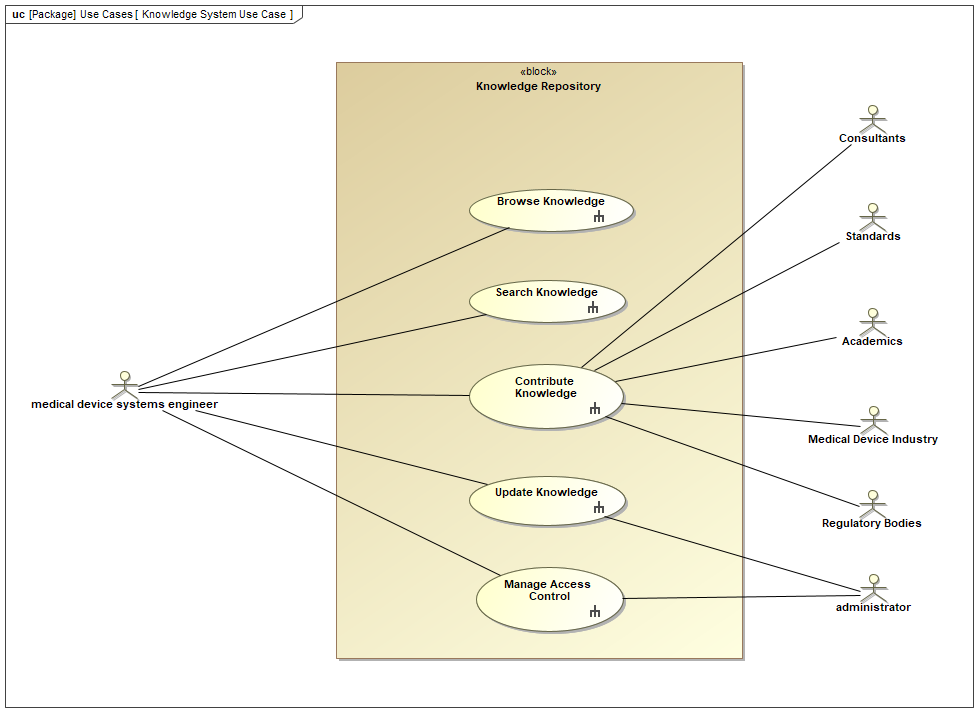
\includegraphics{images/paste-2.png}

\subsection{Collaboration and Knowledge
Sharing}\label{collaboration-and-knowledge-sharing}

The presence of diverse actors and their associated use cases highlights
the collaborative nature of the knowledge repository system. The system
fosters knowledge sharing within the medical device industry, allowing
engineers, consultants, and regulatory bodies to access and contribute
valuable information. Academics and standards bodies can also benefit by
leveraging the repository for research and standard development
purposes.

The SysML use case diagram demonstrates a well-defined knowledge
repository system designed to facilitate knowledge sharing and
management within the medical device industry. The diverse set of actors
and their associated use cases emphasize the system's potential to serve
a wide range of stakeholders. Future analysis could explore the system's
internal structure, including its knowledge representation and retrieval
mechanisms, to provide a more comprehensive understanding of its
functionality.

\section{System Sequences}\label{system-sequences}

\subsection{Main System Function
Sequence}\label{main-system-function-sequence}

This section analyzes a SysML sequence diagram representing the
interaction between a medical device systems engineer and a knowledge
repository system. The diagram depicts a knowledge retrieval process
crucial for informed decision-making within the medical device
development domain.

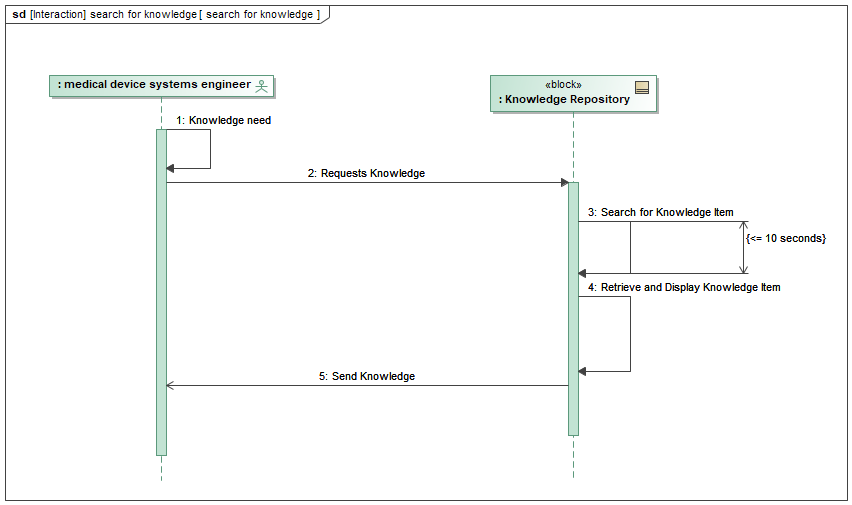
\includegraphics{images/paste-4.png}

\textbf{Actors and Interactions:}

The sequence diagram focuses on two primary actors:

\begin{itemize}
\item
  \textbf{Medical Device Systems Engineer:} This actor represents the
  user of the system, an engineer seeking knowledge pertinent to medical
  device design or development.
\item
  \textbf{Knowledge Repository:} This block represents the system
  component housing the relevant knowledge base for medical devices.
\end{itemize}

The interaction commences with the activation of the \textbf{Medical
Device Systems Engineer}. This signifies the engineer encountering a
\textbf{knowledge need}, prompting them to initiate a search within the
knowledge repository. The engineer transmits a request to the knowledge
repository, likely specifying the desired knowledge domain or specific
keywords related to their need.

\textbf{Knowledge Retrieval Process:}

Upon receiving the request, the knowledge repository executes a
\textbf{Search for Knowledge Item} operation. This operation signifies
the system's internal process of identifying relevant knowledge within
its storage. The diagram incorporates a time constraint, indicating that
the search should be completed within 10 seconds or less. This
emphasizes the system's prioritization of search efficiency, ensuring
timely knowledge retrieval for the engineer.

Following a successful search, the knowledge repository retrieves the
identified knowledge item. This retrieved item could encompass various
formats such as technical references, design guidelines, or regulatory
guidelines relevant to medical devices. Finally, the knowledge
repository transmits the retrieved knowledge item back to the engineer,
enabling them to analyze the information and utilize it to address their
specific knowledge need.

\textbf{Significance for Medical Device Development:}

This SysML sequence diagram offers a simplified yet insightful
representation of a critical interaction within the medical device
development process. Efficient access to relevant knowledge empowers
engineers to make informed decisions concerning design, development, and
regulatory compliance. The time constraint on the search operation
underscores the importance of a well-structured and indexed knowledge
repository, facilitating rapid retrieval of necessary information.

\textbf{Further Considerations:}

While this diagram provides a foundational understanding of the
knowledge search process, further exploration could involve:

\begin{itemize}
\item
  Investigating alternative interaction scenarios, such as browsing by
  category or utilizing advanced search functionalities.
\item
  Analyzing potential error conditions during the search process and the
  system's response mechanisms.
\item
  Considering the knowledge repository's internal structure and indexing
  methods for efficient retrieval.
\end{itemize}

By delving deeper into these aspects, a more comprehensive understanding
of the knowledge retrieval system and its impact on informed
decision-making within the medical device development domain can be
achieved.

\subsection{Update Content Sequence}\label{update-content-sequence}

This following sequence diagram demonstrates a simplified content update
process within the knowledge repository system. It highlights the
interaction between the engineer and the knowledge repository, but
doesn't show details like content format validation or error handling.

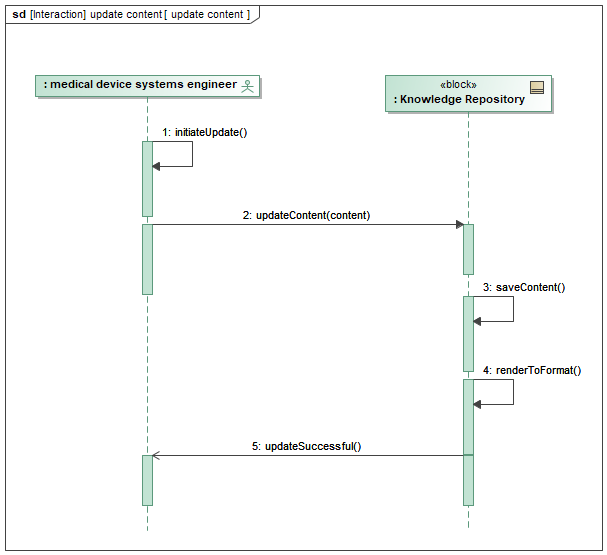
\includegraphics{images/paste-5.png}

The image depicts a SysML sequence diagram for updating content in the
knowledge repository system. The diagram showcases the interaction
between a medical device systems engineer and the knowledge repository.

Here's a breakdown of the interaction sequence:

\begin{enumerate}
\def\labelenumi{\arabic{enumi}.}
\item
  The \texttt{medical\ device\ systems\ engineer} initiates the update
  process by calling the \texttt{initiateUpdate()} function.
\item
  The \texttt{knowledge\ repository} receives the
  \texttt{initiateUpdate()} call and responds with the
  \texttt{updateContent(content)} function, prompting the engineer to
  provide the new content.
\item
  The engineer provides the content through the
  \texttt{updateContent(content)} function call.
\item
  The \texttt{knowledge\ repository} then performs the
  \texttt{saveContent()} function to store the updated content.
\item
  After successful update, the \texttt{knowledge\ repository} sends a
  confirmation message through the \texttt{updateSuccessful()} function.
\end{enumerate}

\bookmarksetup{startatroot}

\chapter{Physical Architecture}\label{physical-architecture}

\section{Top Level System Breakdown}\label{top-level-system-breakdown}

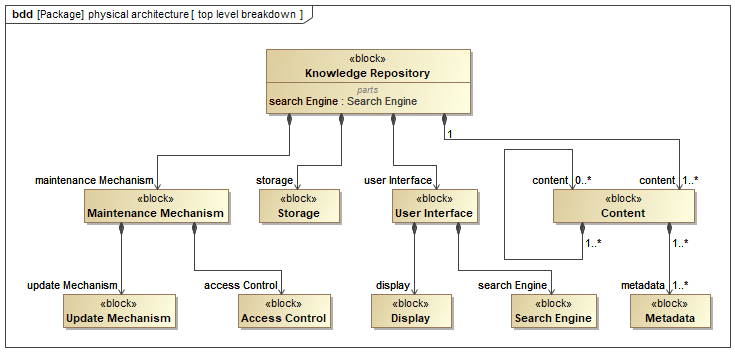
\includegraphics{images/paste-1.png}

The image is a SysML block definition diagram (BDD) for a physical
architecture. It shows the breakdown of a system into its parts at a
high level. Here's a breakdown of the components:

\begin{itemize}
\item
  \textbf{Knowledge Repository:} This block stores knowledge, the data
  that the system operates on.
\item
  \textbf{Search Engine:} This block finds information within the
  knowledge repository. It takes a search query as input and provides
  results.
\item
  \textbf{Maintenance Mechanism:} This block is responsible for
  maintaining the system. It includes an update mechanism and access
  control.

  \begin{itemize}
  \item
    \textbf{Update Mechanism:} This block updates the knowledge
    repository.
  \item
    \textbf{Access Control:} This block controls access to the system,
    by authenticating users.
  \end{itemize}
\item
  \textbf{Storage:} This block stores data, the knowledge repository or
  other system data.
\item
  \textbf{User Interface:} This block allows users to interact with the
  system. It provides content to the user and can receive content from
  the user.
\item
  \textbf{Display:} This block presents information to the user.
\item
  \textbf{Content:} This block refers to the data that is presented by
  the user interface and displayed.
\item
  \textbf{Metadata:} This block provides data about other blocks in the
  system.
\end{itemize}

The diagram also shows the relationships between these blocks. For
example, the search engine has a part relationship with the knowledge
repository. This means that the search engine is a component of the
knowledge repository. The user interface also has a content relationship
with the content block. This means that the user interface displays
content.

\bookmarksetup{startatroot}

\chapter*{References}\label{references}
\addcontentsline{toc}{chapter}{References}

\markboth{References}{References}

\phantomsection\label{refs}
\begin{CSLReferences}{1}{0}
\bibitem[\citeproctext]{ref-incose_incose_2023}
INCOSE, ed. 2023. \emph{{INCOSE} Systems Engineering Handbook}. 5th
edition. Hoboken, {NJ}: Wiley.

\bibitem[\citeproctext]{ref-knuth84}
Knuth, Donald E. 1984. {``Literate Programming.''} \emph{Comput. J.} 27
(2): 97--111. \url{https://doi.org/10.1093/comjnl/27.2.97}.

\end{CSLReferences}



\end{document}
